\section{Problema 2: A medias}

\subsection{Descripción de la problemática}
En este problema se nos pide calcular todas las medianas parciales, que se obtienen al tomar subconjuntos del original de la siguiente manera:
Suponiendo que tengo el siguiente conjunto $\{2,8,5,3,10\}$, tomamos los subconjuntos
\begin{center}
	$\{2\}$ $\{2,8\}$ $\{2,8,5\}$ $\{2,8,5,3\}$ $\{2,8,5,3,10\}$
\end{center}
Luego- entendiendo la mediana como el valor en la posición central o el promedio entre los dos valores en las posiciones centrales (en el caso que la cantidad de elementos sea par) de un conjunto de datos ordenados - la calculamos para cada uno de esos subconjuntos. De esta manera, con el algoritmo que analizaremos a continuación, podemos obtener el siguiente conjunto de medianas $\{2,5,5,4,5\}$ que es solución al problema y que cumple que el $i$-ésimo, con $i = \{0 $..$ 4\}$, representa la parte entera de la mediana de los primeros $i$ números de la entrada.

\subsection{Resolución propuesta y justificación}

La solución que proponemos utiliza dos heaps (uno que ordena los elementos de menor a mayor -min heap- y el otro de mayor a menor -max heap-) para obtener de forma rápida los elementos que se encuentran en la mitad del conjunto ordenado. Para lograr esto, el algoritmo almacena los elementos mas grandes en el min heap y los mas chicos en el max heap, decidiendo si es mas chico o mas grande al compararlo con la mediana del subconjunto anterior.\\

El pseudocódigo que se muestra a continuación representa nuestro algoritmo y en el mismo se utilizan las variables $heap1$ y $heap2$ solamente para mostrar que estamos comparando los dos heaps y que no importa diferenciar cual es el max y cual es el min heap.\\

Pseudocódigo:
\begin{algorithmic}
	\STATE $mediana =$ mediana actual (inicializada en cero)
	\FOR{Cantidad de elementos en el conjunto}
		\IF{Valor del elemento actual $\geq mediana$}
			\STATE Insertar el valor en el min heap
		\ELSE
			\STATE Insertar el valor en el max heap
		\ENDIF
		%balancear heaps
		\IF{La diferencia absoluta entre los tamaños de los dos heaps $>$ 1}
			\STATE Pasar la cabeza del heap mas grande al otro heap
		\ENDIF

		%calcular mediana
		\IF{Tamaño del $heap1 =$ tamaño del $heap2$}
			\STATE $mediana = $ el promedio entre las cabezas de los heaps
		\ELSE
			\STATE $mediana = $ la cabeza del heap mas grande
		\ENDIF
		\STATE Devolver $mediana$
	\ENDFOR
\end{algorithmic}


Los heaps se encargan de mantener ordenadas las dos mitades del conjunto, pero como no se sabe de antemano contra que valor comparar para ubicar los elementos en el heap correcto, los mismos se pueden debalancear, generando que los elementos del medio no se encuentren en las cabezas. Por este motivo si llega a ocurrir ese caso, balanceamos los heaps pasando la cabeza del heap mas grande al otro.\\

Luego calcular la mediana simplemente implica decidir si el subconjunto actual tiene cantidad par o impar de elementos y en función de eso, calcular el promedio de las dos cabezas o tomar la cabeza del heap mas grande.

Por el invariante del ciclo \emph{for}: \texttt{\{$i >= 0 \land i <$ cantidad de elementos del conjunto $\land\ mediana =$ mediana de los primero $i$ números\}}, podemos asegurar que el ciclo termina, ya que se cumple antes y después de cada iteración del ciclo y al darse la condición de terminación (\texttt{$i >=$ cantidad de elementos del conjunto}), efectivamente termina. Luego por la documentación de \emph{Priority Queue} sabemos que los heaps van a mantener los elementos ordenado en todo momento, dándonos fácil acceso al mínimo y el máximo. Al rebalancear los heaps nos aseguramos de que siempre se cumpla que la diferencia absoluta entre los tamaños de los heaps sea menor igual a uno, lo que causa que los heaps tengan la mitad o la mitad mas uno de los elementos del subconjunto actual. Teniendo en cuenta que vale lo anterior y por estar ordenados de forma ascendente el que contiene los elementos más pequeños y de forma descendente el otro, se cumple que las cabezas siempre representan a los elementos centrales del subconjunto actual con $j$ elementos, o sea, los valores en las posiciones $j/2 \land (j/2)+1$. Por lo que para calcular la mediana podemos obtener los tamaños de los heaps y decidir si hay que calcular el promedio o devolver la cabeza del mas grande. De esta manera el algoritmo cumple con la definición de mediana para cada subconjunto incremental.

\subsection{Análisis de la complejidad}
Nuestra solución tiene una complejidad temporal de $\mathcal{O}(n\log{}n)$ siendo $n$ la cantidad de elementos del conjunto. \\

El algoritmo está contenido en un \emph{for} que recorre una sola vez cada elemento del conjunto, con lo cual la ejecución de ese ciclo tiene una complejidad de $\mathcal{O}(n)$. Luego se utilizan los métodos de la clase \emph{Heap} que utiliza como base a la clase \emph{Priority Queue} que está incluida en \emph{java.util}. Las complejidades de todos los métodos de \emph{Priority Queue} que se mencionan a continuación, están especificadas en la documentación de java\footnote{http://docs.oracle.com/javase/7/docs/api/java/util/PriorityQueue.html}. El algoritmo ejecuta los métodos de \emph{Heap} de la siguiente manera:

\begin{itemize}
	\item Insertar elemento en heap: Es $\mathcal{O}(1)$ elegir en que heap se va a insertar el elemento mas $\mathcal{O}(\log{}n)$ insertar en la cola de prioridad con \emph{PriorityQueue.add()}.\\ Notar que el elemento nunca se inserta en los dos heaps, por lo tanto la complejidad queda\\ $\mathcal{O}(1) + \mathcal{O}(\log{}n) = \mathcal{O}(\log{}n)$.
	\item Balancear heaps: Hace comparaciones y asignaciones en $\mathcal{O}(1)$, luego llama a \emph{PriorityQueue.poll()} que obtiene y remueve la cabeza del heap en $\mathcal{O}(\log{}n)$ y por último inserta la cabeza en el otro heap con \emph{PriorityQueue.add()} también en $\mathcal{O}(\log{}n)$.\\ Quedando una complejidad de $k * \mathcal{O}(1) + 2 * \mathcal{O}(\log{}n) = \mathcal{O}(\log{}n)$ con $k$ una constante.
	\item Calcular mediana: Hace operaciones aritméticas, asignaciones y comparaciones en $\mathcal{O}(1)$, obtiene los tamaños de los heaps con \emph{PriorityQueue.size()} también en $\mathcal{O}(1)$ y obtiene la cabeza de uno o de los dos heaps, lo cual no hace diferencia ya que la complejidad de \emph{PriorityQueue.peek()} es $\mathcal{O}(1)$.\\ En este paso nos queda una complejidad de $k * \mathcal{O}(1) = \mathcal{O}(1)$ con $k$ una constante.
\end{itemize}

\noindent Por lo tanto, siguiendo el análisis de complejidad, nos termina quedando:
\begin{center}
	$\mathcal{O}(n) * (\mathcal{O}(\log{}n) + \mathcal{O}(\log{}n) + \mathcal{O}(1)) = \mathcal{O}(n\log{}n)$
\end{center}
Lo cual condice la afirmación que hicimos al principio de la sección.

\newpage
\subsection{Código fuente}
\lstinputlisting[name=AMedias, numbers=left, frame=lines, firstline=30, lastline=47]{../src/ej2/src/Main.java}
\lstinputlisting[name=Heaps, numbers=left, frame=lines, firstline=7, lastline=18]{../src/ej2/src/Heap.java}
\lstinputlisting[name=AMedias, numbers=left, frame=lines, firstline=20, lastline=38]{../src/ej2/src/Heap.java}
\lstinputlisting[name=AMedias, numbers=left, frame=lines, firstline=40, lastline=52]{../src/ej2/src/Heap.java}

\subsection{Experimentación}

\subsubsection{Constrastación Empírica de la complejidad}
\begin{figure}[h!]
   \begin{center}
 	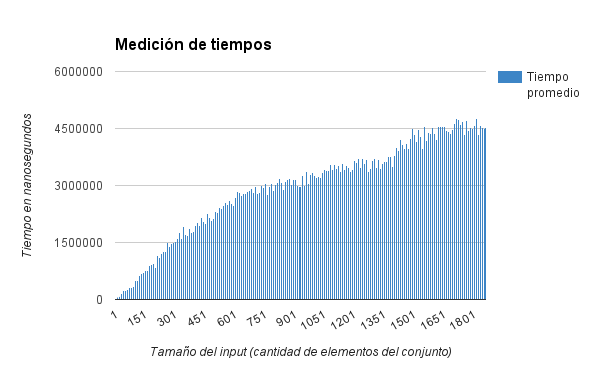
\includegraphics[scale=0.8]{imagenes/ej2/tiempos.png}
	\caption{Medición de tiempo promedio entre 100 corridas}
	\label{estacionesRel}
   \end{center}
 \end{figure}

 \begin{figure}[h!]
   \begin{center}
 	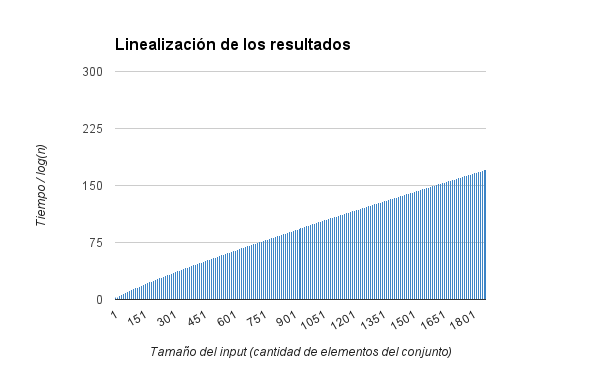
\includegraphics[scale=0.8]{imagenes/ej2/linealizacion.png}
	\caption{Tiempo promedio dividido por la cota de complejidad}
	\label{estacionesRel}
   \end{center}
 \end{figure}

